\chapter{標準、標準英語、そして何を教えるべきか}\label{sec:standards}\label{ch:standards}

\begin{tblsframedsymbol}{学習目標}{bulb}
  \begin{itemize}[noitemsep, leftmargin=*]
      \item 品質としての \mention{standard} と慣習としての \mention{standard} の違いを区別する
      \item 標準英語（Standard English）を単一の強固なものではなく、関連する変種（varieties）の集まりとして認識する
      \item 標準英語が他の直言（dialects）よりも本質的に優れているわけではないことを理解する
      \item 文法性（grammaticality）と有意味性（meaningfulness）の違いを分析する
      \item 文法性に関する直感がなぜ当てにならないことがあるのかを理解する
      \item 処理の限界が文法性の判断にどのように影響するかを認識する
      \item 形式と意味のペアリング（form--meaning pairing）の分析を適用して、文法的な容認可能性（acceptability）を理解する
      \item 文法規範（grammatical norms）を定義する上での言語共同体（speech communities）の役割を理解する
      \item 文法に対する記述的（descriptive）アプローチと規範的（prescriptive）アプローチを区別する
  \end{itemize}
  \end{tblsframedsymbol}

\section{はじめに}
\hyperref[ch:categories]{次の章}では、語彙範疇の説明に戻りますが、ここでは、英語に関して何が正しく何が間違っているかという認識に関連するいくつかの問題について少し考える時間を割くべきでしょう。この章は、\term{標準（standards）}\is{standard|(}、\term{標準英語（Standard English(es)）}\is{Standard English|(}、\term{文法性（grammaticality）}\is{grammaticality|(}、そして\term{規範性（normativity）}\is{normativity|(}の概念について考えるのに役立つはずです。これらはすべて、英語教師が理解しておくべき重要な概念です。

なぜこれらの概念が重要なのでしょうか？教師として、私たちは英語において何が\enquote{正しい}かという裁定者になることをよく求められます。しかし、これから見ていくように、それは常に見た目ほど単純なことではありません。何が標準でしょうか？何が文法的でしょうか？そしておそらく最も重要なこととして、私たちは実際に何を教えるべきでしょうか？

まず、\enquote{標準}という概念を解きほぐし、それが言語にどのように適用されるかを見ていきます。次に、標準英語、より正確には複数の標準英語の概念と、なぜこの区別が重要なのかを探ります。さらに、文法性\is{grammaticality!questioning of|(}について深く掘り下げ、何が文法的\is{grammatical!vs meaningful|(}または非文法的\is{ungrammaticality}であるか、そしてこれに関する私たちの直感\is{intuition!about grammaticality|(}がなぜ時として誤解を招くことがあるのかを検証します。最後に、言語の規範的な側面と、それが教師としての私たちの決定にどのような影響を与えるかを考察します。

この章が終わる頃には、これらの概念についてよりニュアンスに富んだ理解を得て、英語教育という複雑な風景をナビゲートする準備がより整っているはずです。それでは、私たちが何かが\enquote{標準}であると言うときに何を意味するのかを考えることから始めましょう。

ほとんどの人にとって、\mention{standard} は肯定的な含意\is{standard!positive connotations of}を持っています。\mention{standard} と一緒に使う言葉、たとえば \mention{gold standard} と \mention{quality standard}、あるいは \mention{standard of living} と \mention{standard of care} といったペアを考えてみてください。高い基準を持っていたり、それを超えたりするのは良いことです。私たちは教育の基準、環境の基準、技術の基準\is{technology standard}\is{technology standard|(}を設定しますが、これらはすべて私たちの教育、環境、技術をより良くするためのものです。

要するに、標準とは私たちが目指すものであり、\term{標準英語（Standard English）}（大文字の \mention{S} に注目してください）は目指すべきもののように聞こえるかもしれません。それは\enquote{良い}英語、文法的な\is{grammatical!vs Standard English|(}英語、あるいは文学的な英語と同等だと思うかもしれません。しかし、定義したり目標にしたりするのは、それほど単純でも明確でも簡単なことではありません。

あなたはおそらくVHSが何であるかを知っている年齢でしょう。しかし、ベータマックス（Betamax）が何であるかを知るには若すぎるかもしれません。一時期、これらは競合するビデオテープの規格でした。ほとんどの基準で、ベータマックスの方が高品質な製品でした。画質も音質も優れていました。しかし、それは随分前に消滅したため、あなたは聞いたことすらないかもしれません。そしてVHSがビデオカセットテープとプレーヤーの標準となりました（少なくとも人々がまだVCRを使っていた間は）。

標準は良いという意味ではありませんし、良いからといって標準というわけでもありません。

さまざまな軌間（レールの幅）が存在しますが（図~\ref{fig:rail}）、標準軌\is{standard!rail gauge analogy}は幅1.435メートルです。私が住んでいるミシサガ（Mississauga）の新しいライトレール路線にはこれが使われています。しかし、東隣の都市であるトロントのトロント交通局（TTC）で伝統的に使われているトロント軌間は、幅1.495メートルです。確かにそれぞれのサイズには長所と短所がありますが、標準軌の最大の利点は、それが標準であるということです。最も一般的に使用されているため、新しい鉄道車両や中古の鉄道車両を必要とする場合、標準軌を使用する方がはるかに安く、早く手に入ります。これが、トロントのシステムと直接車両を互換させることができなくなるにもかかわらず、ミシサガがそれを選んだ理由です。この選択は品質や優位性に関するものではなく、コストと可用性に関するものでした。

標準英語\is{Standard English!not inherently superior|(}は英語の\enquote{最高}の形態ではありません。標準英語が他の方言\is{dialect!and Standard English|(}よりも本質的に優れているわけではありません。標準英語は単に、最も広く受け入れられ、最も制度化され、多様なコミュニケーション\is{communication!as function of language}のための最も一般的な共通基盤であるに過ぎません。

言語学において、\mention{standard} という言葉は、質的な指標というよりも、むしろ社会政治的な指標\is{Standard English!as a sociopolitical marker}として機能することがよくあります。それは、歴史的、文化的、そしてしばしば植民地主義的な力によって、ある方言（通常は社会的または経済的に支配的なグループの方言）が他の方言よりも引き上げられた結果なのです。

ですから、私たちが標準英語について語るとき、本当に議論しているのは、体系化され、学校で教えられ、公文書で使用され、正式な場で期待される一連の慣習のことなのです。それは知性、道徳性、あるいは価値の尺度ではありません。単に最も一般的かつ広範に期待され、受け入れられているものに過ぎません。そして、それはほとんどの人々が\enquote{英語を話せるようになりたい}と言うときに心に抱くものです。標準英語における \mention{standard} という言葉は、品質に関するものではなく、むしろ偏在性と制度的な後ろ盾に関するものです。それは英語という言語におけるVHSであり、必ずしもベータマックスではないのです。

\begin{figure}
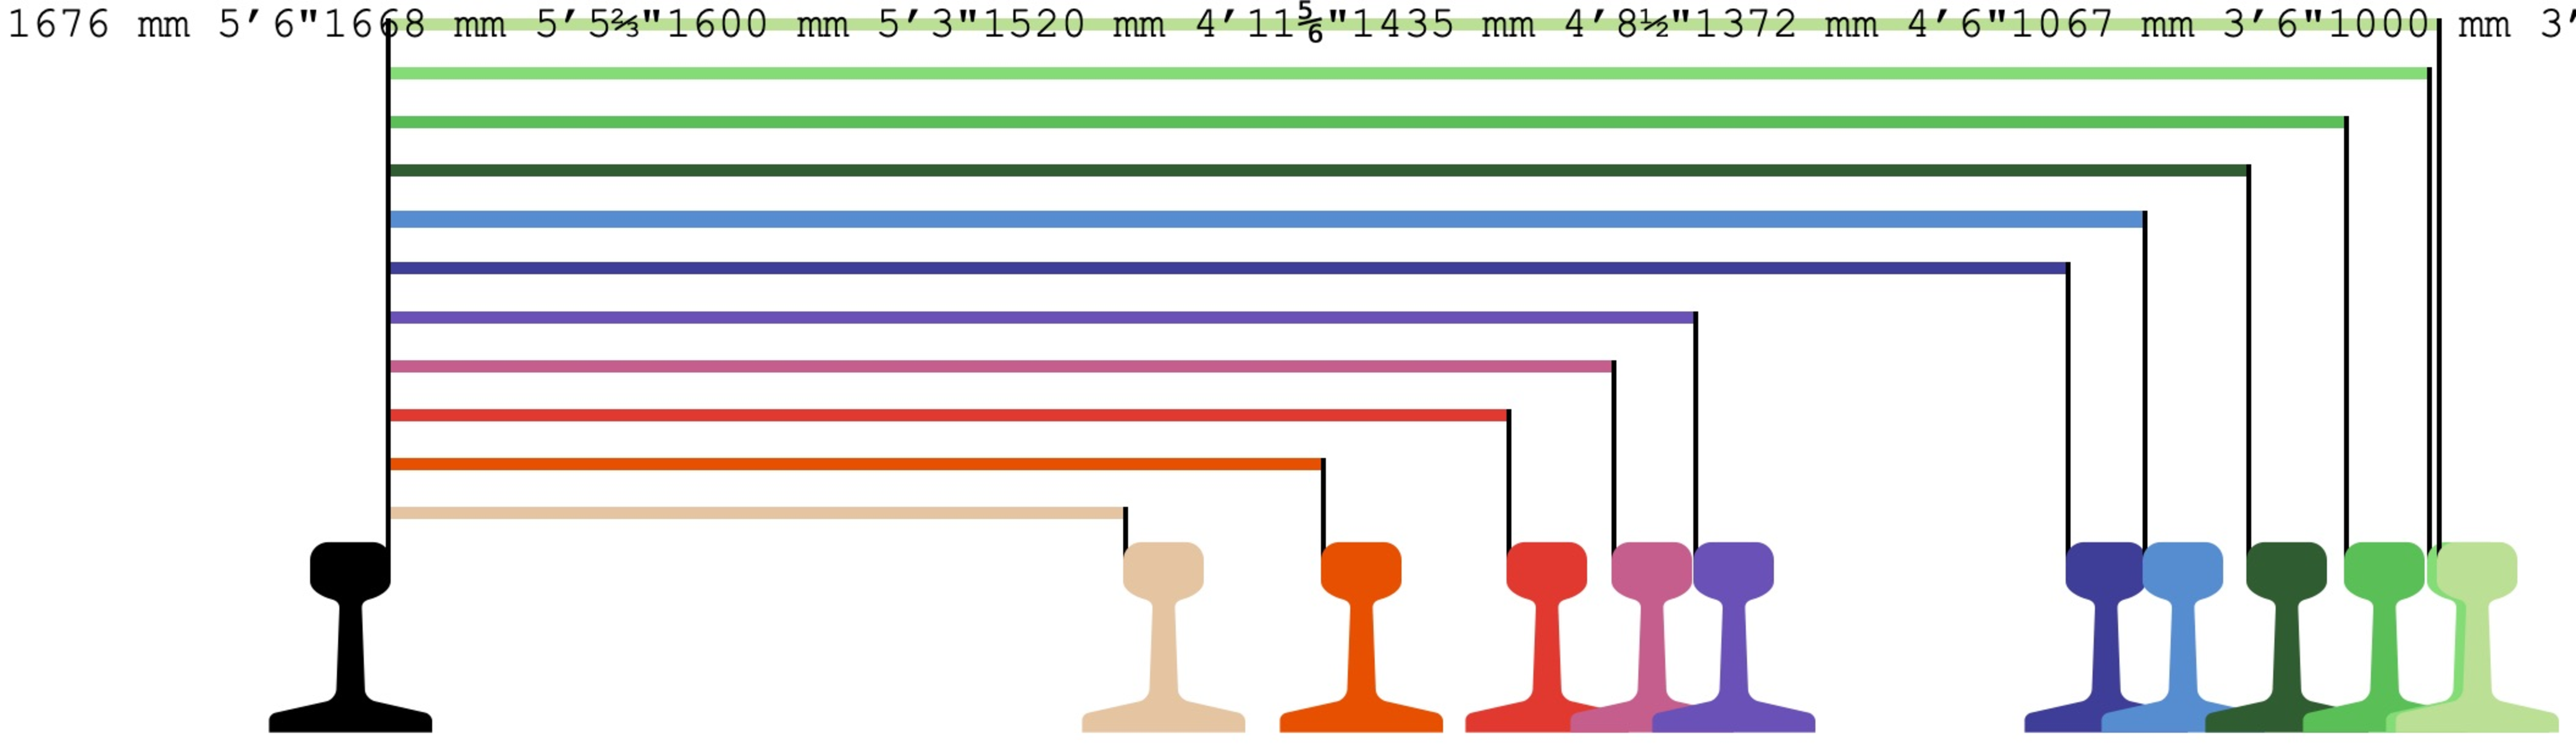
\includegraphics[width=0.7\textwidth]{figures/Track_gauge.pdf}
\caption{軌間}
\label{fig:rail}
\end{figure}

標準は現代世界を支えていますが、しばしば恣意的\is{standard!arbitrary nature of|(}なものです。A4用紙は世界のほとんどの地域で標準であるため、そこではA4がより優れています。USレターサイズは北米の標準であるため、そこではUSレターがより優れています。どちらも本質的に優れているわけではありません。その優位性は、標準であることから来ているのです。

標準英語もこのパターンに従っています。本質的に優れているのではなく、標準であるから優れているのです。他の多くの英語も、もし標準であったならば、標準になり得たのです。

しかし、技術の基準\is{technology standard!vs language standards|(}と言語の基準\is{language standard!vs technology standards|(}には2つの重要な違いがあります。第一に、技術基準は規定されるものです。誰かが計画を立て、それを公表したのです。言語はそのようなものではありません。第二に、技術基準に従わなければ、技術はしばしば機能しません。たとえば、TTCの路面電車は標準軌のレール上では全く走りません。交通手段として使い物にならないのです。同様に、VHSカセットはベータマックスのプレーヤーでは全く再生できません。対照的に、非標準の英語は、標準英語の話者が相手であっても、コミュニケーション\is{communication!and non-standard English}の手段として完全に機能することが多々あります（おそらくほとんどの場合）。私たちが理解できない、あるいは簡単に理解できない方言や変種もありますが、私たちが理解できるものはそれ以上にたくさんあります。コミュニケーションが言語の主な機能であるならば、なぜ私たちは標準英語を持っているのでしょうか？

1つの答えは、言語のもう1つの機能がグループメンバーシップ\is{group membership!and dialect|(}を規定することだということです。言い換えれば、言語は私たちに似ている人、私たちのグループに属している人を特定するのに役立ちます。若者はしばしばスラングを開発し、革新し、使用することで、仲間内のグループ内でアイデンティティや帰属意識を生み出します。たとえば、\enquote{素晴らしい}を意味する形容詞としての \mention{fire} は、一時期、一部の若い話者の間で人気を集めました。そのように使用した人々は、\enquote{私は \mention{fire} のこの新しい意味を知っているグループの一員だ}と宣言しており、さらに\enquote{私はあなたに対してそれを使うから、あなたもそのグループの一員だと思っている}という意味も込めていました。もちろん、大人がそのグループの一部になることはめったになく、大人が \mention{fire} をそのように使うこともめったにありませんでした。

あるいは服装について考えてみてください。カナダのほとんどのカレッジや大学では、ジーンズが標準です。スーツやドレスを着る人もいますが、これらはよりフォーマルではあるものの、依然として標準的な服装の範疇です。教室が暖かければ、上半身裸で現れることも完全に機能的かもしれませんが、それは標準ではありません。人々はそのような服装の選択に対して、驚きや不快感を持って反応するでしょう。スノースーツも非標準ですし、サリー、シェフのユニフォーム、男性のキルトも同様です。キャンパスの人々の中には肯定的に反応する人もいれば否定的に反応する人もいるでしょう。多くの人は表面的な反応を抑えるでしょうが、誰もがこれらの服装が非標準であると認識するはずです。

非標準の英語に関しても同じようなことが言えます。あなたがそれを使えば、人々は気づきます。標準英語は社会的な基準であり、社会的な意味合いを持っています。通常、標準英語を話さない人にとってそれは否定的なものであり、語学教師として、私たちは生徒たちの目標が道具的であると同時に社会的でもあることを認識すべきです。彼らは社会で機能するために英語を学びたいと思っていますが、同時に社会の一部になるために標準英語を学びたいと思っているのです\is{standard!arbitrary nature of|)}\is{technology standard|)}。


\section{標準英語（Standard Englishes）}\label{sec:standard}

ジョージ・エリオットは、彼女の小説『ミドルマーチ』の中で次のような会話を提示しています。

\begin{quote}
    \enquote{All choice of words is slang. It marks a class.}（言葉の選択はすべてスラングだ。それは階級を示している。）

    \enquote{There is correct English: that is not slang.}（正しい英語というものがある。それはスラングではない。）

    \enquote{I beg your pardon: correct English is the slang of prigs who write history and essays. And the strongest slang of all is the slang of poets.}（失礼ですが、正しい英語とは、歴史やエッセイを書く堅物たちのスラングです。そして最も強力なスラングは、詩人たちのスラングです。）
\end{quote}


エリオットは\enquote{正しい英語}と標準英語の違いを知っていました。しかし、多くの人は知りません。残念ながら、私がそれを明確にするために使えるような、標準英語の簡潔な定義\is{Standard English!definition (lack of brief)}はありません（ここでも定義の難しさがあります）。実際、本書の1つの目標は、標準英語の統語論、語彙、および音韻論の限定的な定義を概説することです。しかし、その支配的な地位について、少なくともいくつかコメントすることはできます。

ある程度、英語のどの方言も、あるグループの間では標準ですが、そのほとんどは\enquote{標準英語}とは呼ばれません。もしあなたが標準軌の列車をTTCの地下鉄向けに売ろうとしても、売れることはないでしょう。標準軌はトロントで使用されている標準ではないからです。

もしあなたがファースト・ネーションズ英語\is{dialect!First-Nations English}を話して育ったなら、あなたのコミュニティではファースト・ネーションズ英語がおそらく標準です。あなたのコミュニティに行って標準英語を話す人は誰でも、自らをよそ者として際立たせることになり、良くも悪くもそのように扱われるでしょう。

そして明確にしておきたいのは、標準英語は1つではないということです。カナダ標準英語\is{Standard English!Canadian}、イギリス標準英語\is{Standard English!British}、シンガポール標準英語\is{Standard English!Singapore}などが存在します。大部分において、少なくとも書き言葉にされた場合、これらはほとんど区別がつきませんが、小さな違いはあります。ある変種の独自の特徴は、別の変種の話者にはしばしば目につくものです。それでも、これらはすべて標準英語として、あるいは最近では複数の標準英語として認識されています。

しかし繰り返しますが、これは標準英語が優れているからでも、よりフォーマルだからでも、あるいは最も一般的だからでもありません（特定のコミュニティにおいて最も一般的ではありますが）。\footnote{標準英語が\enquote{何ではないか}についての詳細は、\citet{trudgill99} を参照してください。}\mention{standard} という言葉は、\mention{grammatical} や \mention{correct} の同義語ではありません。真実、論理、美しさ、純粋さ、あるいは明晰さを暗に意味するものでもありません。それは英語がどのように話される\enquote{べき}かということではありません。それは単なる方言の集まり\is{Standard English!as a cluster of dialects}であり（強力なものではありますが）、英語話者の支配的な社会的グループによって施行されている規範に過ぎないのです。世界の多くの地域で、それはイギリスや、先住民が大部分追いやられた旧イギリス植民地（例：カナダ）の教育を受けた英語話者を意味しますが、先住民が追いやられなかった場所（例：バングラデシュ）の話者は含まれません\is{Standard English!not inherently superior|)}\is{dialect!and Standard English|)}。

\begin{tblsframed}{\term{シボレス（shibboleth）}\is{shibboleth|(}とは何か？} \label{sec:shibboleth}
    ヘブライ語聖書の7番目の書である士師記には、方言の門番としての機能\is{shibboleth!gate-keeping function}に関する物語があり、次のような内容です。

    \begin{quote}
        エフタはギレアデのすべての人を集めてエフライムと戦った。ギレアデの人々はエフライムを打ち破った。エフライムが、\enquote{あなたがたギレアデは、エフライムとマナセの間にあるエフライムの逃亡者だ}と言ったからである。
        ギレアデはエフライムへ行くヨルダン川の渡し場を攻め取った。エフライムの逃亡者が、\enquote{渡らせてくれ}と言うと、ギレアデの人々は、\enquote{おまえはエフライム人か}と問い、彼が\enquote{違う}と答えると、
        彼らは、\enquote{それでは \mention{Shibboleth}（シボレス）と言ってみろ}と言った。彼がそのとおりに正しく発音できず、\enquote{Sibboleth}と言うと、彼らは彼を捕らえ、ヨルダン川の渡し場で彼を殺した。その時、エフライムは四万二千人倒れた。 --士師記 12:4-6 (新改訳聖書をもとに調整)
    \end{quote}

    \indent この物語から、英語の \mention{shibboleth}\is{shibboleth!origin of term} という言葉が生まれました。これは特定のグループの人々を区別する話し方であり、しばしばアイデンティティの確認や帰属のテストとして使用されます。\mention{shibboleth} という用語は現在、\enquote{インサイダー}と\enquote{アウトサイダー}を分けるあらゆる種類の言語的または文化的指標を意味します。現代の用法において、シボレスは生と死の問題ではないかもしれませんが、それでも私たちが他者をどのように認識し、どのように接するかに大きな影響を与える可能性があります。

\end{tblsframed}

\section{文法性への問い} \label{sec:questioning-grammaticality}

私が初めて英語教師として雇われたとき、それは私の資格のせいではありませんでした。私には何の資格もありませんでした。また、経験のせいでもありませんでした。先ほど言ったように、それが私の最初の教職だったからです。それでも、私が日本に到着したとき、2週間以内に雇われました。これはおそらく私が標準英語の\enquote{ネイティブスピーカー}であったからだと推測しています。白人であることもおそらく役立ったのでしょう。

標準英語を話して育った人間として、私は明らかにこの言語の有能な使い手でしたが、明示的な文法知識はほとんど持っていませんでした。カナダのほとんどの学校は、英文法について本質的に何も教えません。それは私が学生だった頃もそうでしたし、現在でもそうです。私はフレンチ・イマージョンの初期の波の中にいたため幸運でした。少なくとも（フランス語の）文法について何かを知っていたからです。しかし、生徒たちの質問に答えようとしたとき、それはほんのわずかな助けにしかなりませんでした。

\enquote{なぜここでは現在進行形を使い、あちらでは現在形を使うのですか？}、\enquote{いつ \mention{the} が必要ですか？}、\enquote{なぜ \mention{who \emph{does} she know} とは聞くのに、通常 \mention{who \emph{does} know her} とは聞かないのですか？}これらのすべての質問に対して、私は\enquote{そう言う方が自然に聞こえるから}以上のことはほとんど言えませんでした。私は何が文法的で何が非文法的かについて強い直感\is{intuition!about grammaticality}を持っていましたが、それらの直感を体系的かつ一般化可能な方法で生徒たちに伝える術を持っていませんでした。そもそも、何かが文法的であるとはどういう意味なのかについて考えたことすらありませんでした。

この時点で、あなた（そうです、あなたです）は、かつての私よりもずっと多くの英語文法の明示的な知識をすでに持っています。実際、あなたはおそらく平均的な大学教授よりも英文法に関する明示的な知識を持っています。もし生徒が \mention{I had coffee and a piece of toast for breakfast} の中の限定詞について尋ねてきたら、\mention{coffee} は不可算名詞なので限定詞を必要としないが、単数の可算名詞である \mention{piece} は限定詞なしでは使えないと教えることができるでしょう（セクション~\ref{sec:count} を参照）。あなたは英文法について何かを知っています。ですから、私が始めた頃よりもずっと先を行っているのです。

しかし、あなたもまた、何かが文法的であるとはどういう意味なのかについて考えたことがないかもしれません。これがここで探求したいことです。（より完全な扱いは第\ref{ch:grammaticality}章で行います。）

\begin{tblsframed}{\term{単義性の誤謬（The fallacy of monosemy）}\is{fallacy of monosemy|(}} \label{sec:fallacy-of-monosemy}\is{monosemy}
    しかし、本題に入る前に、単義性の誤謬について一言述べておきます。もしある単語が単義的であれば、それは単一の（\mention{mono--}）意味（\textit{\emph{sem}antics}）を持っています。これは、子供が\enquote{\mention{can I go to the toilet}}と尋ねたときに、教師が意地悪く\enquote{\mention{I don't know, \emph{can} you?}}と答えるときに働いている考え方です。教師は \mention{can} が\enquote{能力}というたった1つの意味しか持たないかのように振る舞っていますが、実際には \mention{can} は複数の意味を持っています。第1章で、専門的な意味と日常的な意味について触れました。誰かが\enquote{専門的にはその単語は $x$ を意味する}と言うとき、単にその単語の専門的な意味合いが存在すると言っているだけかもしれませんが、多くの場合は単義性の誤謬に陥っているのです。
\end{tblsframed}\label{sec:monosemy}

\mention{grammatical} という言葉にたった1つの真の意味があると見せかける必要はありませんが、だからといって何でも意味するわけではありません。\mention{grammatical} の意味をどのように確立するのでしょうか？図~\ref{fig:comic} のコミックが説明しているように、言葉が何を意味するかは、私たちがそれを使うときに何を意味するかに依存しています。

ですから、あなたにとって \mention{grammatical} と \mention{ungrammatical} が何を意味するのか少し時間をかけて考えてみてください。あなたがこれらの言葉を使ったときのことを思い出してください。あなたは何を指していましたか？もし思い浮かばなければ、それぞれの例を作ってみてください。いずれにせよ、他の例にも一般化できるかもしれない共通点を考えてみてください。特に境界事例が思い浮かんだ場合は重要です。

\begin{figure}
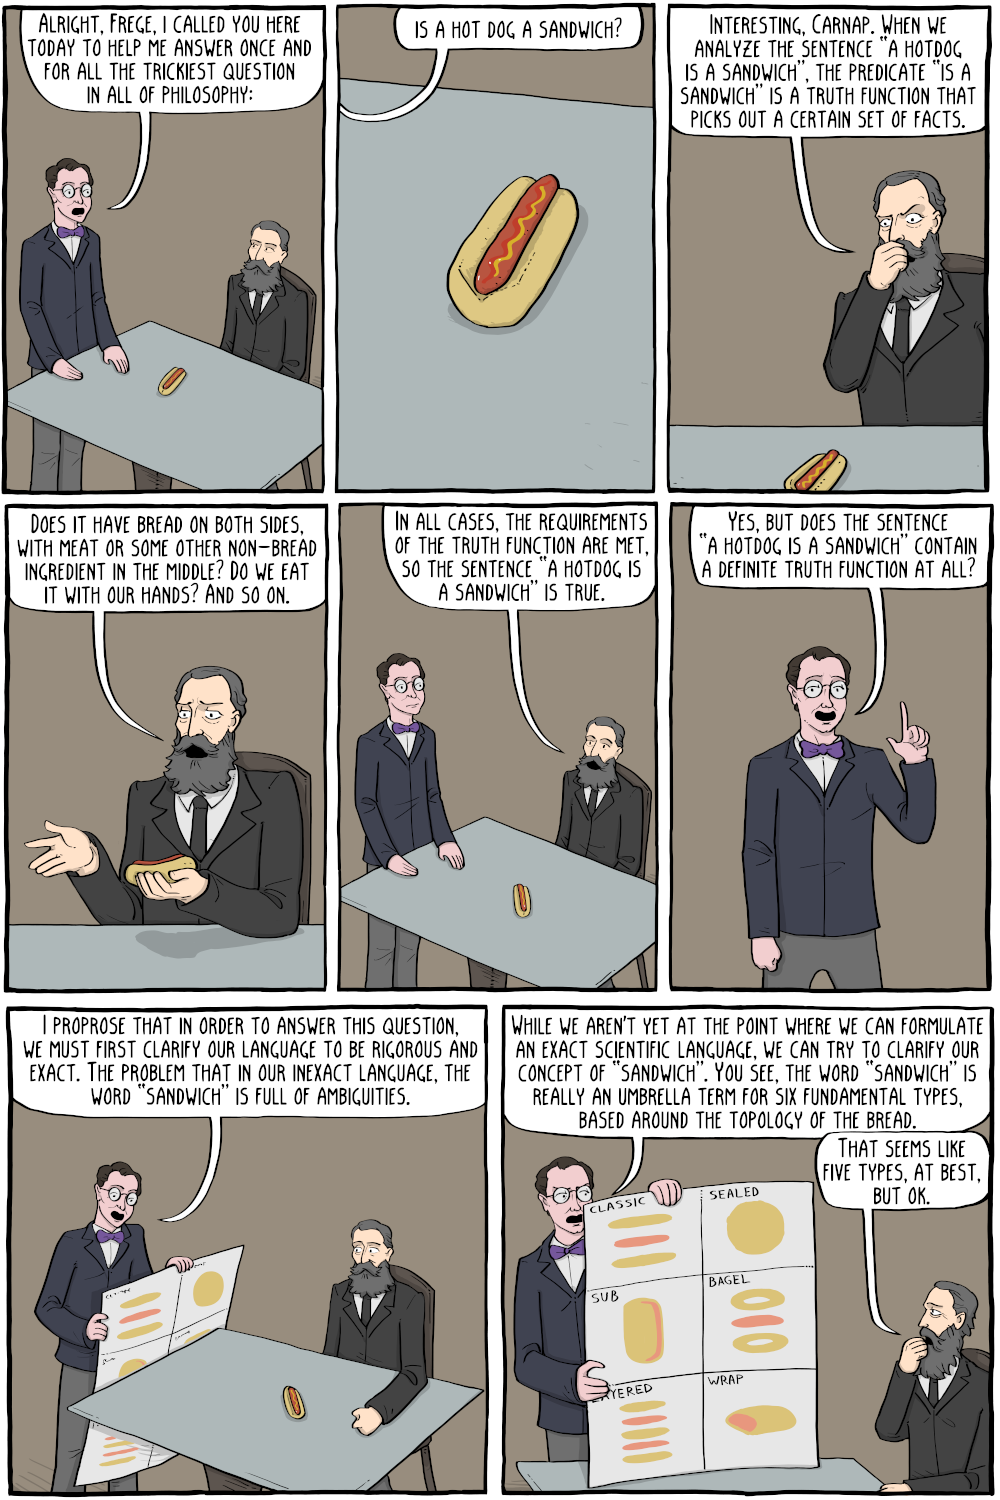
\includegraphics[width=0.95\textwidth]{figures/hotdogSandwich1.png}
\end{figure}

\begin{figure}
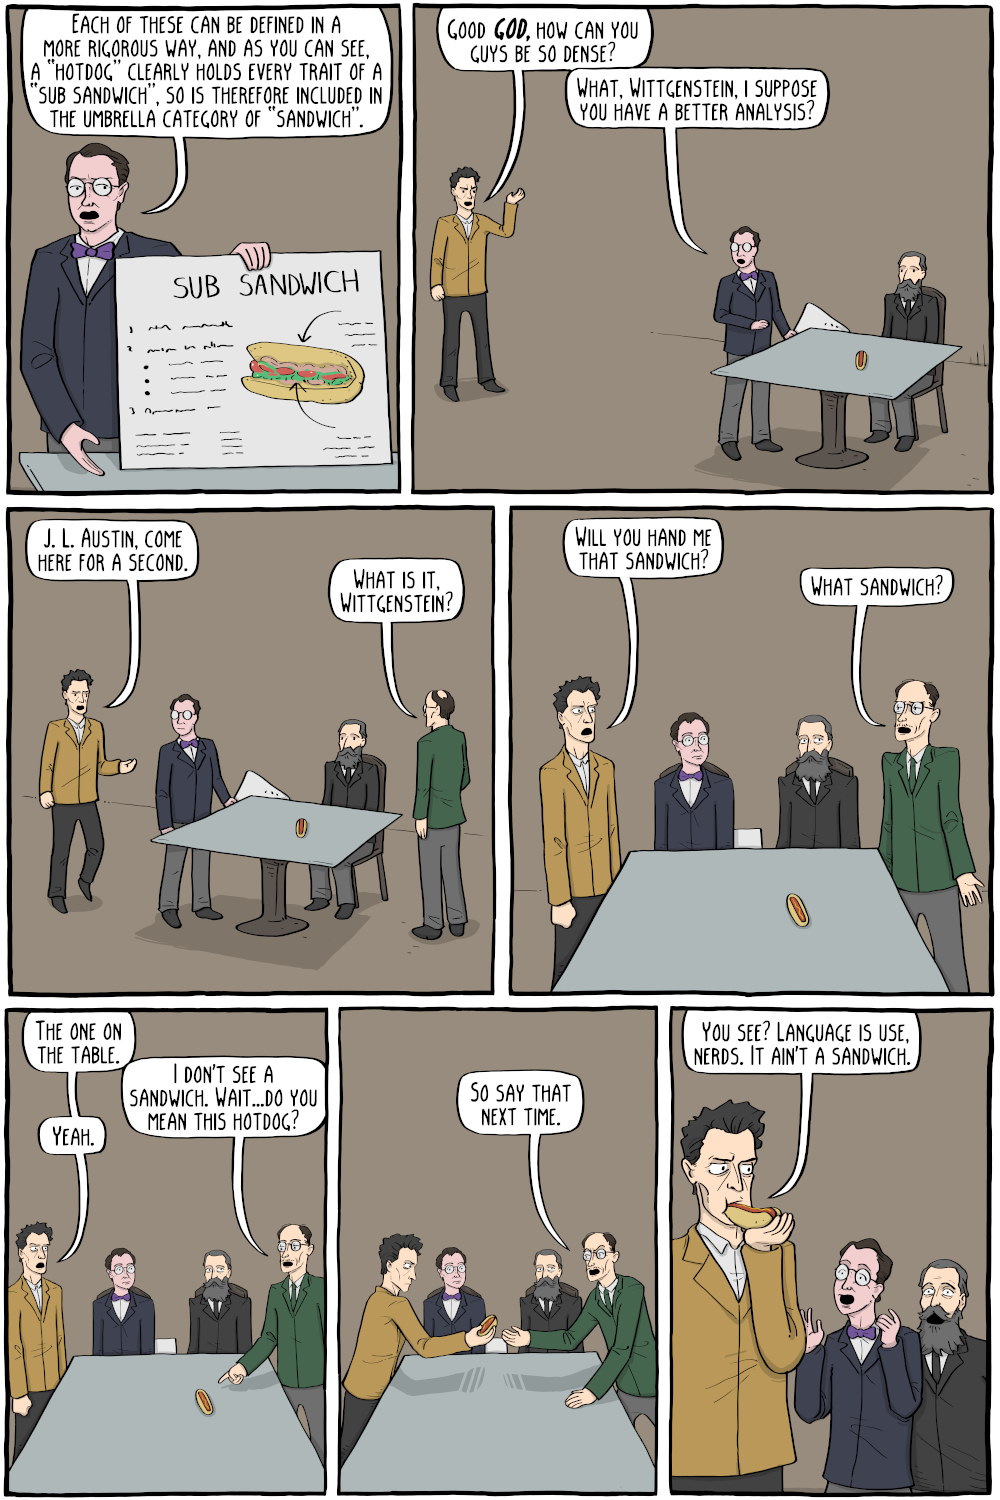
\includegraphics[width=0.90\textwidth]{figures/hotdogSandwich2.png}
\caption{Is a Hotdog a Sandwich? A Definitive Study, from \textit{Existential Comics} by Corey Mohler.}
Source: \url{https://existentialcomics.com/}
\label{fig:comic}
\end{figure}

\textit{The concise Oxford dictionary of linguistics} \citep{Matthews2003} では、\mention{grammatical} を次のように定義しています。


\begin{enumerate}[noitemsep]
    \item 文法に関すること [\dots]。
    \item 特に、ある言語の規則に従っている文などについて。例：英語において \mention{I like tea} は文法的であるが、\mention{I tea like} は非文法的である。したがって、文法性\is{grammaticality!definition}は、特定の文法によって文に割り当てられる特性、あるいはその文法を仮定的に\enquote{知っている}話者によって容認可能であると判断される文の特性のいずれかである。
\end{enumerate}

言語とは単なる使用であるというウィトゲンシュタインの概念に行き着くのでしょうか？私たちが話すことはすべて文法的であるということでしょうか？私たちの発話が私たちの文法を定義するのでしょうか？まあ、そうですが、それはあなたやあなたの生徒の役には立たないので、いくつかの例を考えてみたいと思います。

簡単なものから始めましょう。


\ea[]{Me key there happy mine the.}
\label{ex:key}
\z
(\ref{ex:key}) が紛れもなく非文法的\is{ungrammaticality!example of|(}であることに同意していただけると思います。しかし、なぜでしょうか？いや、本当に、なぜでしょうか？もしあなたがこれが非文法的だと感じるなら、その直感を裏付けるために何を指摘できますか？もし誰かがこれが実際には文法的だと主張したら、私たちはどのような反論ができるでしょうか？

さて、\mention{key} から始めて、それが単数の可算名詞であるため限定詞が必要であり、それがないように見えると言えるかもしれません（セクション~\ref{sec:count} を参照）。\mention{my} のようなNPは限定詞として機能できますが、少なくとも標準英語において \mention{me} はそのようには機能しません。おそらくこれは \mention{me} が\enquote{私の}を意味する別の方言の \mention{me} かもしれませんが。あなたは \mention{key} を見て、それが名詞なのか動詞なのかを自問するかもしれません。もしそれが名詞なら、動詞はありません。そしてもしこれが節であるべきなら、主要部としてVPが必要です（セクション~\ref{sec:verbs} を参照）。そこで、\mention{key} が動詞だと仮定しましょう。そうなると \mention{me} が主語になりますが、ここでは \mention{me} ではなく \mention{I} が期待されます。そして \mention{key} が動詞なら、あなたは何かをキーで傷つける（key something）ことを期待します。残念ながら、\mention{there} と \mention{happy} はキーで傷つけられる\enquote{何か}ではありません。\mention{please key mine} と言うことはできますが、それが機能するためには \mention{mine} が \mention{key} から離れすぎているように思えます。そして \mention{the} は、通常決して現れない位置である文末に残されています。

私は続けることができますが、おそらくもっと単純なことです。もしかすると (\ref{ex:key}) は意味をなさないから非文法的なのかもしれません。文法的な言語は常に意味をなすものなのでしょうか？意味をなすものは文法的だと言えるでしょうか？（これらは同じ主張ではありません。）批判的思考を持つ者として、私たちは自分のアイデアを反証しようとする必要があります。意味をなさない文法的な発話を作成し、非文法的な発話と比較することでこれを行うことができます。幸いなことに、言語学において非常に影響力のあるノーム・チョムスキーが、(\ref{ex:greenIdeas}) の有名な（少なくとも言語学においては）例でそれをすでに行ってくれています。

\ea
    \ea[]{Colorless green ideas sleep furiously.}
    \label{ex:greenIdeas1}
    \ex[*]{Furiously ideas sleep green colorless.}
    \label{ex:greenIdeas2}
    \z
    \label{ex:greenIdeas}
\z

\begin{figure}
    
\includegraphics[width=3in]{figures/green-ideas.png}
    \caption{Colorless green ideas sleep furiously.}
    \label{fig:greenIdeas}
\end{figure}

\textcite[16]{Chomsky2002-ko} は、(\ref{ex:greenIdeas1}) は文法的であり、(\ref{ex:greenIdeas2}) は非文法的であると主張しています。これは私の直感と一致します（あなたの直感とも一致すると思います）。文法的であるために意味をなす必要はないようです。


しかしチョムスキーはまた、これらの文やその部分が英語のコーパスに出現することはなく、\enquote{英語のいかなる統計モデルにおいても、英語から同等に『かけ離れて』いる}と主張しています。彼は、頻度は関係ないと言いたいのです。ここにおいて、彼は間違っていると思います。フェルナンド・ペレイラ（Fernando \textcite{Pereira2000}）は、(\ref{ex:greenIdeas1}) が実際には (\ref{ex:greenIdeas2}) よりも統計的にずっと起こりやすいことを示しました。そして ChatGPT のような大規模言語モデルの成功は、言語が統計的規則性\is{grammaticality!and statistics}の上に構築されていることを真に示しています \citep{Kallini2024}。

次に、その逆である、有意味な言語はすべて文法的であるということを検討します。それを行う前に、非文法的であるが明確な意味を持つものを何か考えてみてください。

さて、(\ref{ex:JeanPaul}) を考えてみてください。

\ea[]{Jean Paul, very very good.}
\label{ex:JeanPaul}
\z
この例は私の友人であるジェフ・プラムがNPRのインタビューで聞いたものです。話者はトルコ人でした。その文脈における彼女の意味は明らかに、教皇ヨハネ・パウロが非常に、非常に良い教皇または人物であったということでした。しかし、これが英語で文法的であるためには、主語と主要部を持つ節が必要です。その主要部はVPであるべきで、つまり動詞が必要になります。おそらく \mention{be} でしょうが、\mention{seem} や \mention{become} のような叙述補語を認可する他の動詞も可能でしょう。

つまり、何かが文法的であっても意味をなさない\is{grammatical!vs meaningful}ことがあり、意味をなすけれども文法的ではない\is{meaning!and grammaticality|(}ことがあるようです。したがって、意味は文法性のための必要条件でも十分条件でもありません。\is{necessary and sufficient conditions}

それでは、別の考えです。おそらく私たちは文法書の規則\is{grammaticality!and rule books}にただ従えばいいのではないでしょうか。

\ea
    \ea[]{He was a beautiful young man, a beautiful beautiful boy.}\label{ex:beautifulboy}
    \ex[*]{The boy was beautiful beautiful.}\label{ex:beautifulboy2}
    \z
\z
星印（*）でわかるように、私は (\ref{ex:beautifulboy}) は文法的だと思いますが、(\ref{ex:beautifulboy2}) はそうではないと思います。あなたも同意してくれると思います。これを説明する規則は \textit{CGEL} (p. 561) にあり、私の知る限り \textcite{Watt1968} によって最初に注目されました。しかし、それは広く知られておらず、あなたもこれまでに遭遇したことはないと思います。また、(\ref{ex:beautifulboy}) と (\ref{ex:beautifulboy2}) の文法性が、Watt が論文を書いたときから \textit{CGEL} が出版されるまでの間に変わったわけでもないと仮定します。これらのことを考慮すると、文法書の規則が何が文法的かを規定するという考えは脇に置いておくことができるでしょう。多くの規則は文法書に言及されていません。実際、言語学者がそのための文法書を一切書くことなく存在している言語がたくさんあります。本が書かれていないからといって、それらの言語では何でもありだと言いたくはないはずです。

さて、(\ref{ex:whmovement}) を考えてみてください。

\ea[*]{What movies do you have friends who acted in?}
\label{ex:whmovement}
\z
おそらくこれは非常に奇妙な文で、文法的であると同時に非文法的であるように感じる、まるで目の錯覚のような文だということに同意するでしょう。その理由は、\term{島の制約（island constraints）}\is{island constraint}と呼ばれるものによる結果だと考えられています。これは、これに関して議論はありますが、多くの言語学者がすべての言語に適用されるかもしれないと考えている一種の規則または制限です。これは私たちの脳の処理の制約\is{processing limitations!and grammaticality|(}による結果である可能性もありますし、情報がどのように構造化されるかに関する何かである可能性もあります。幸いなことに、もしこれが真実であれば、あなたはこれを生徒に説明する必要は決してないでしょう。なぜなら、誰も素朴にこのような文を使おうとはしないからです。

つまり、私たちの処理能力が、何が文法的で何がそうでないかを判断するのに役立っているようです。これを念頭に置いて、(\ref{ex:suitcase}) が図~\ref{fig:suitcases} のどちらの画像を説明しているか考えてみてください。

\ea[]{After the trip, my suitcase sat unpacked on the floor for days.}
\label{ex:suitcase}
\z

\begin{figure}
    
\includegraphics[width=2in]{figures/full_suitcase.png}
    
\includegraphics[width=2in]{figures/empty_suitcase.png}
    \caption{どちらのスーツケースが unpacked ですか？}
    \label{fig:suitcases}
\end{figure}

多くの人は、これは最初のスーツケース（左側の服が入っているもの）だと言いますが、それは間違いです。最初のスーツケースは \mention{packed} です。スーツケースを \mention{pack} するとき、あなたは服を中に入れます。2番目のものは \mention{unpacked} されています。すべての服が取り出されているのです。

なぜ人はこれを間違えるのでしょうか？この問題について考えた人々は、否定、つまり \mention{unpacked} の先頭にある \mention{un--} に何か巧妙な罠があると感じることがよくあります。結局のところ、それを \mention{packed} に置き換えれば、意味は完全に明確になります。では、私たちの言語処理の方法に、時折私たちの理解を混乱させるある種のバグがあるのでしょうか？もしかすると、何が文法的かを判断するために直感に頼ることは全くできないのかもしれません。実際、これはまさに (\ref{ex:horse}) が示唆していることです。

\ea[]{The horse raced past the barn fell.}
\label{ex:horse}
\z
言語学で有名なもう1つの文である (\ref{ex:horse}) は、おそらくあなたには非文法的に思えると思いますが（\citet{bever1971} より）、星印（*）がないことにお気づきかもしれません。\mention{raced} を \mention{ridden} に変えたらどうでしょうか？今度は明らかに文法的です（もし明確でなければ、これは\enquote{納屋を通り過ぎて走らされたその馬は転んだ}という意味です）。あなたが (\ref{ex:horse}) で抱えた問題は、\mention{raced} を過去分詞形（\mention{ridden} のような）ではなく、過去形（\mention{rode} のような）として解釈したことでした。やはり、私たちの直感は100\%信頼できるわけではないのかもしれません。時として、一歩一歩慎重に考え抜く必要があります。

(\ref{ex:30years}) に関して言えば、これは完全に文法的であるように私には思えます（比較：\mention{I have 30 dollars}）。実際、多くの言語において年齢はこのように語られます。しかし、それが文法的であったとしても、少なくとも英語において \mention{I'm 30 years old} と言う方法としては間違っています。ですから、文法的であることさえも、容認可能\is{grammatical!vs acceptable}であることと同じではないのです。
\ea[\textsuperscript{?}]{I have 30 years.}
\label{ex:30years}
\z
北米の英語話者は一般的に (\ref{ex:weekend}) を非文法的だと判断しますが、これはイギリス英語において \mention{I'll see you on the weekend} を表現する通常の方法です。

\ea[\textsuperscript{!}]{I'll see you at the weekend.}
\label{ex:weekend}
\z
これはセクション~\ref{sec:standard}で触れた、標準英語間の小さな違い\is{Standard English!regional differences}の1つであり、\enquote{!}のマークはそれが標準英語の変種間で異なることを示しています。この違いの理由は文法的なものではなく、週末に関する関連するメタファー\is{metaphor!for weekend (platform vs point)}について異なる文化的前提の下で操作しているためです。北米人は週末を出来事が展開するプラットフォームや舞台として捉えているのに対し、イギリス人は週末を週の終わりにある点として見ていると主張されています。\footnote{メタファーと前置詞についての詳細は、セクション~\ref{sec:preposition-meanings} を参照してください。}

\ea[\textsuperscript{\%}]{I ain't no quitter.}
\label{ex:quitter}
\z
(\ref{ex:weekend}) とは異なり、(\ref{ex:quitter}) は標準英語間の違いではありません。\enquote{\%}のマークは、標準英語では文法的ではないかもしれないが、他の変種では文法的である形式を示しています。

\ea[]{Me and Mia are taking the bus.}
\label{ex:bus}
\z
対照的に、(\ref{ex:bus}) はすべての方言において完全に文法的ですが、インフォーマルな使用域\is{style restrictions (formal, informal, etc.)!and register}に属しています。よりフォーマルなバージョンでは \mention{Mia and I} を使用します。これは一部の人々にとってのシボレス\is{shibboleth!example of}です。

最後に、私が非文法的だと感じる (\ref{ex:bad-and}) を修正してみてください。
\ea[*]{Jim and me's teacher was Geoff.}
\label{ex:bad-and}
\z
ここには良い解決策がありません。もしそれを \mention{Jim and my} に変えれば、それは\enquote{私の先生とジム}のようになり、私が意味していることではありません。\mention{me and Jim's} にも同様の問題が当てはまります。しかし、*\mention{Jim and my's} は *\mention{Jim and me's} と同じくらい非文法的に聞こえます。特定の単純な概念を表現するために、時には非文法的である必要があるのかもしれません。私はそうしたケースがあるかもしれないと考えています\is{ungrammaticality!example of|)}\is{fallacy of monosemy|)}\is{intuition!about grammaticality|)}\is{meaning!and grammaticality|)}\is{processing limitations!and grammaticality|)}\is{grammaticality!questioning of|)}\is{grammatical!vs meaningful|)}。

\subsection{まとめ}

一般的に、文法的なものは意味をなし、その逆もまた然りですが、意味をなすことは文法性のための必要条件でも十分条件でもありません。規則の多くは文法書に記述されていますが、多くは記述されていません（そしてしばしば文法書の記述は間違っています）。英語の熟練した使用者は、何が文法的かを知るために概ね直感に頼ることができますが、私たちの直感は騙されることがあります\is{intuition!fallibility of|(}。時には、説明が以前には見えなかったものを見るのに役立つこともあります。文法的なものでも私たちが言わないようなことがあり、また文法的に言うことができないこともあります。それでは、文法的なものを文法的にしているのは何でしょうか？

\section{文法性のモデル} \label{sec:gramm-model}

さて、文法性は私たちが思っていたほど単純ではないことを見てきました。しかし、だからといって文法性について有用な考え方ができないというわけではありません。役立つかもしれないモデル\is{grammaticality!model of|(}をここに示します。

その核心において、文法性とは、特定の状況における特定のスピーカーグループに対して機能する形式と意味のペアリング\is{form--meaning!pairing|(}に関するものです。それは普遍的なものではありません。図~\ref{fig:speaker_groups} は、それらのグループのほんの一部を示しています。私が言いたいことを理解するために、10代の若者が\enquote{それはあなたのお母さんの靴下だ}という意味で \mention{mommy sock} と言うことを考えてみてください。これは非常に非文法的に（そして非常に奇妙に）感じられます。しかし、幼児による同じ発話は、どちらの感情も呼び起こしません。なぜなら、それは特定の状況における特定のスピーカーグループに対して機能する、適切な形式と意味のペアリングだからです。

あるいは、\citet[179]{nishimura1995} からの次の会話を考えてみてください。斜体のテキストは日本語\il{Japanese}で、単一引用符の中に翻訳があります。

\begin{quote}
    B.C. \mention{ni iku toki} (`When I went to B.C.'), \mention{hikōki de yomoo to omotte kara} (`thinking I would read it on the plane'), I bought it, eh? So, it's not finished yet. (Laughs) And it's hard, 'cause me\mention{-nanka} (`a person like me'), \mention{mō} (`really'), \mention{hon-nanka yomu to} (`when I read a book'), cover-to-cover \mention{yomanakattara} (`unless I read it cover-to-cover'), if I stop \mention{dokka de }(`at some point'), I forget the story.\\
    （B.C.に行く時、飛行機で読もうと思ってから、買ったのね。だから、まだ終わってないの。（笑）そして難しいの、だって私なんか、もう、本なんか読むと、カバーからカバーまで読まなかったら、どっかで止めたら、話を忘れちゃうの。）
\end{quote}

このような\term{コードスイッチング（code-switching）}\is{code-switching!and grammaticality}\is{code-switching!example of}は、英語と日本語のバイリンガルにとっては完全に文法的ですが、他の英語話者にとっては大部分が非文法的に思えます。

\begin{figure} \label{fig:speaker-groups}
\begin{tikzpicture}[scale=0.8]
    % Main ellipse for all English speakers
    \draw[fill=white, thick] (0,0) ellipse (7cm and 5cm);
    \node[align=center] at (0,4.2) {All English Speakers\\（すべての英語話者）};

    % Ellipse for Standard English speakers
    \draw[fill=white, thick] (-1,0) ellipse (5cm and 3cm);
    \node[align=center] at (-1,2.3) {Standard English Speakers\\（標準英語話者）};

    % Smaller ellipses for different groups
    \draw[fill=white, thick] (-3,-1) circle (1.2cm);
    \node[align=center] at (-3,-1) {Teachers\\（教師）};

    \draw[fill=white, thick] (0,-2) circle (1.2cm);
    \node[align=center] at (0,-2) {Teens\\（10代）};

    \draw[fill=white, thick] (2.7,0.9) circle (1.3cm);
    \node[align=center] at (2.7,0.9) {Singaporeans\\（シンガポール人）};

    \draw[fill=white, thick] (4,-2) circle (1.2cm);
    \node[align=center] at (4,-2) {Infants\\（幼児）};

    \draw[fill=white, thick] (-4.2,1.3) circle (1cm);
    \node[align=center] at (-4.2,1.3) {Lawyers\\（弁護士）};

    \draw[fill=white, thick] (-4.2,-4) circle (1.5cm);
    \node[align=center] at (-4.2,-4) {People in 1300\\（1300年の人々）};

\end{tikzpicture}
\caption{英語話者のグループ間の関係（縮尺は正確ではありません）。}
\label{fig:speaker_groups}
\end{figure}


意味\is{meaning!context-dependent|(}に関していえば、それを伝えるために使用される構文と一致する必要がある層が何層にも重なっていることがよくあります。\mention{Try it and you'll regret it} には文字通りの意味\is{meaning!literal vs implied}があります。それは何かを試すという指示の後に、その経験が後悔につながるという述定が続くというものです。しかし、日常会話では、それは条件的な意味を持ちます。\enquote{もしあなたがそれを試せば、あなたは後悔するだろう}。それらの上に、暗黙の脅しを伴うこともあります。\enquote{もしあなたがそれをしたら、私はあなたを罰する}。ここでは、命令形の \mention{try it} の文字通りの意味が覆され、\enquote{それを試すな}という意味になります。

時として、古い構文が新しい意味とペアになることがあります。私たちが \mention{going to} による未来時間の慣用表現を最終的に持つようになったのはそのためです。それは何かをするためにどこかへ行くこと（例：\mention{Why am I going there? I'm going to shop.}）という文字通りの意味から始まりましたが、その活動がある程度の移動時間の後にしか起こり得ないという事実が、それが未来の意味を帯びる機会を提供したのです。またある時は、文法的な構文がより非文法的になったり、使われなくなったりします。たとえば、英語での疑問文や否定文の作り方を見てください。シェイクスピアは \mention{don't you know?} の代わりに \mention{know you not?} と尋ねたでしょうし、明らかにそれはあなたや私の言い方ではありません。



では、私たちはいつ何かが非文法的だと言うのでしょうか？いくつかの状況が思い浮かびます。第一に、形式が意味と全くペアにならない、あるいはいかなる意味も示唆しない場合です（例：\mention{Can the have running?}）。第二に、あなたが意図することと、人々があなたに意図していると期待することの間にミスマッチがある場合です。\mention{I have 12 years} は、\mention{How long do you have until retirement?} という質問に答える方法としては完全に良いものですが、\mention{How old are you?} という質問に対する答えとしては非文法的\is{ungrammaticality!conditions for|(}です。


第三に、同じ発話の中に矛盾する形式と意味のペア\is{form--meaning!pairing!contradictory}がある場合です。\mention{I have two job} は、その仕事の数が複数であることと、それが単数であることを同時に私たちに伝えています。そして最後に、強く好まれる代替形式があり、それを使用しない明確な理由がない場合です。

\mention{It's very good} のような一般的なフレーズを考えてみましょう。ほとんどの英語話者はこれを文法的と呼ぶでしょう。代わりに \mention{It very good} と言っても、意味は伝わります。結局のところ、非文法的であることは無意味であることを意味しません。しかし、聞き手はなぜあなたが動詞を飛ばしたのかと不思議に思い、言葉を詰まらせるかもしれません。何かを引用しているのでしょうか？ミームを参照しているのでしょうか？珍しい形式に対する明確な理由がなければ、彼らはそれを非文法的だと判断する可能性が高いでしょう。

これらの判断は、常に信頼できるガイドというわけではありません。私たちの脳は時として、処理が複雑だという理由だけで、完全に文法的な文に\enquote{間違っている}というフラグを立てることがあります。また、特に意味に集中しているカジュアルな会話の中では、実際に非文法的なフレーズに気づかずに通り過ぎてしまうこともあります。

このモデルは、文法性を、文法書から規則に従うこととしてではなく、特定の文脈\is{context!and grammaticality|(}においてあなたの言語共同体で機能する形式と意味のペアを使用することとして構成しています。1950年代以降の多くの言語学者が主張してきたことにもかかわらず、文法は私たちの脳に組み込まれているわけではありません。\footnote{たとえば、\citet{chomsky1981lectures} が主張したような生得的な原理とパラメーターを私たちは持っていません。}言語は流動的であり、その話者によって形作られます。何が文法的とみなされるかは、時間、空間、および社会的グループを越えて変化します。

ほとんどの学習者は、標準英語を話す世界に向けて自分のスピーチの目標を定めます \citep[e.g.,][]{Rezaei2019}。誰もがこれらの標準に正確に一致する必要があったり、それを望んだりしているわけではありません。多くの人は、たとえばベトナムのような国でビジネスを行うために、ただ効果的にコミュニケーションを取りたいだけかもしれません。生徒が標準英語を追求するとき、私たちは彼らをその目標へと導きます。幸いなことに、厳格な技術的基準とは異なり、言語の基準\is{language standard!flexibility of|(}は壊れることなく曲がります。完全に意味をなしながら、かなりの程度までそこから逸脱することができます。

文法だけで言語がどのように機能するかは決まりません。社会的な期待と価値観は長い影を落とし、人々が\enquote{正しい}と考えるものを静かに形作っています。そしてこれは私たちを規範性へと導きます。社会のルールがどのように言語を通じて波及し、私たちの言葉と世界における私たちの場所の両方を形作っているかということです\is{intuition!fallibility of|)}\is{form--meaning!pairing|)}\is{meaning!context-dependent|)}\is{ungrammaticality!conditions for|)}\is{context!and grammaticality|)}\is{language standard!flexibility of|)}\is{grammaticality!model of|)}。

\section{規範性}\label{sec:normativity}

\term{規範的（normative）}な声明とは、物事がどうであるかではなく、どうあるべきか、あるいはいかなる価値観\is{normativity!definition|(}が与えられた場合にそれがどのようにあることが適切か、を扱うものです。

\begin{table}
        \begin{tabularx}{\textwidth}{XX}
            \lsptoprule
            規範的（Normative） & 実証的（Positive） \\
            \midrule
            テーブルマナーのルール & 物理学の主張 \\
            倫理学 & 整数論 \\
            経済学：希少な資源をどのように分配すべきか & 経済学：私たちが実際に希少な資源をどのように分配しているか \\
            語学教育 & 言語学 \\
            \lspbottomrule
        \end{tabularx}
    \caption{規範的および実証的ドメイン}
\end{table}

ジェフ・プラム（Geoff \textcite[205]{Pullum2019}）は、次のような規範的観察を行っています：
\begin{itemize}[noitemsep]
    \item \enquote{It is not polite to lick your knife}（ナイフを舐めるのは礼儀正しくない）は、ナイフを舐めないための理由を提供します。
    \item \enquote{Torturing children is wrong}（子供を拷問するのは間違っている）は、子供を拷問しないための理由を含意しています。
    \item \enquote{Bach's music is beautiful}（バッハの音楽は美しい）は、バッハのコンサートに行く計画を立てるための理由を示唆しています。
    \item \enquote{Inflation is too low}（インフレ率が低すぎる）は、中央銀行に金利を下げるべきであるとシグナルを送っています。
    \item \enquote{the fact that torturing a child is immoral,}（子供を拷問することは不道徳であるという事実）から、私たちは子供を拷問すべきではないということになります。
\end{itemize}

英文法のルールは規範的なのでしょうか？もしそうなら、人々が英語をどのように話す\enquote{べき}かについて、それらから何を学ぶことができるでしょうか？プラムは次のように観察しています：
\begin{itemize}[noitemsep]
    \item 誰も英語を話す義務を負っていないのだから、一般に、誰が何をすべきか、あるいは何をすべきでないかについては、何も結論づけられません。
    \item 私たちが特定の変種の英語を話しているとみなされたいのであれば、その変種のルールに従うべきです。
\end{itemize}

一方で、単に英語話者とコミュニケーションを取りたいのであれば、私たちが何をすべきかはあまり明確ではありません。

\begin{itemize}[noitemsep]
    \item おそらく私たちは、理解可能\is{comprehensibility}であること、あるいは理解できることを目指すべきでしょう。文法的な正確さは理解可能性を保証するものではなく、非文法的な言語でもこれまで見てきたように理解可能であることはあり得ますが、ほとんどの理解可能な英語は文法的でもあります。
    \item 同様に、おそらく私たちはタイミングよく流暢であることを目指すべきですが、文法的であることへの懸念は、タイミングの良さや流暢さを低下させる可能性があります。
\end{itemize}

\subsection{オーディエンス}

規範性について最後に1つ指摘しておきたいのは、規範性はしばしばその規範が適用される母集団を前提としているということです（図~\ref{fig:speaker_groups} を思い出してください）。もし文法性が、特定の状況における特定のスピーカーグループにとっての、意味、期待されること、そして処理可能性の組み合わせであるならば、話者が誰であるかだけでなく、\term{オーディエンス（audience）}\is{audience|(}が誰であるかも考慮する必要があります。そのオーディエンスがここでの重要な要素であり、英語を学ぶことに関して言えば、オーディエンスはしばしば標準英語話者の社会的グループになります。

しかし、常にそうとは限りません。英語を学ぶ人々の中には、他の非ネイティブスピーカーと、特定の文化グループと、あるいはおそらく自分たちの個人的なネットワーク内でのみコミュニケーションを取りたいと考える人もいるかもしれません。そしてこれらのグループは、標準英語の話者ではないかもしれません。これらの人々にとって、標準英語の規範はそれほど関連性がないかもしれません。彼らは代わりに、自分たちの特定のターゲットオーディエンス内で関連性があり意味のある別の言語規範のセットを習得する必要があるかもしれません。しかし、私たちの生徒が標準英語の話者になることを望んでいる限り、私たち語学教師はそれを促進すべきであることは私には明白に思えます。それでも、そのような生徒であっても、\hyperref[ch:vocabulary]{語彙をさらに学ぶ}ことや\hyperref[ch:fluency]{処理の流暢さを高める}ことの代わりに、標準英語の忠実度のより細かいレベルを掴むことに時間を費やすべきではないでしょう。

前述のように、しばしば高い忠実度が要求される技術的基準とは異なり、言語の基準は、私たちが寛容である限り、言語内で非常に寛容です。したがって、英語学習者は、オーディエンスの基準から大きく逸脱しながらも、非常にうまくコミュニケーション\is{communication!and grammaticality}を取ることができることがよくあります。ヴィヴィアン・クックが観察したように、\enquote{人々は、自分が属していないグループの規範に従うことは期待できません。そのグループが人種、階級、性別、またはその他の特徴によって定義されているかどうかにかかわらずです。ある任意のグループとは異なる話し方をする人々は、より良く、あるいはより悪く話しているのではなく、ただ異なる話し方をしているだけなのです}\citep[194]{Cook1999}。難しいのは、彼らがどれほど異なる話し方をするか、彼らがどれほど帰属したいと望んでいるか、そして私たちがどれほど彼らを受け入れたいと望んでいるかということになるでしょう。

最後に、促進は双方向に進むことができます。標準的な方法は、生徒に順応するよう負担をかけることです。これがほとんどの英語教師が私たちの仕事を見ている方法であり、おそらく私たちの最も中心的な役割です。しかし、もう1つの方法があります。それは、標準英語話者が他の変種の英語の使用者を調整し\is{accommodation!by Standard English speakers}、含め、受け入れ、歓迎するのを助けることです。言うまでもなく、語学教師は一般的にこれをあまり行っていません。多くの人は全く行っていません。しかし、英語教師として、私たちは少なくともその可能性\is{normativity!definition|)}\is{audience|)}を認識しておくべきです。

\section{結論}

標準英語は社会的および経済的な力を持っており、あなたの生徒はそれにアクセスする必要があります。しかし、\enquote{これは正しいか？}という問いは、イエスかノーで答えられる質問であることはめったにありません。答えはコミュニティ、使用域、そして目的に依存します。そして時として、あなたが言える最も有用なことは、ある形式がただ標準であるということだけでなく、なぜそれが標準であるのかということです。それは赤ペンでエラーを直すよりも難しい対話ですが、この章があなたにその対話を行う準備をさせてくれるのです。\is{standard|)}\is{Standard English|)}\is{Standard English|)}\is{grammaticality|)}\is{normativity|)}\is{audience!and grammaticality|)}\is{shibboleth|)}



\noindent 注意：用語は、それらが詳細に議論されている関連するセクションに相互参照されています。



\begin{tblsframedsymbol}{練習問題}{pencil}

\begin{enumerate}[noitemsep, leftmargin=*]
    \item 言語の文脈における\term{標準（standard）}の概念を説明してください。それは\enquote{良い}や\enquote{正しい}という考え方とどのように異なりますか？
    \item 標準英語と複数の標準英語（Standard English\emph{es}）の区別が重要なのはなぜですか？
    \item シボレスの例を挙げ、それが社会的マーカーとしてどのように機能するかを説明してください。
    \item 文法性を判断するために直感だけに頼ることの限界はどのようなものですか？
    \item 本文では、意味は文法性のための必要条件でも十分条件でもないと主張しています。この主張を例を挙げて説明してください。
    \item 特定の状況における特定のスピーカーグループにとって、形式と意味のペアリングが\term{文法的（grammatical）}であるとみなされることに寄与する要因は何ですか？
    \item ある発話が意味を伝えることに成功していても\term{非文法的（ungrammatical）}と見なされるかもしれない状況を説明してください。
    \item オーディエンスの概念は、文法性についての私たちの理解にどのように情報を提供できますか？
    \item 言語の文脈において、\term{規範的（normative）}という用語は何を意味しますか？
    \item 生徒のために標準英語と文法性の複雑さをナビゲートする上での、TESL教師の役割は何ですか？
\end{enumerate}

\end{tblsframedsymbol}

\begin{tblsfilled}{解答のヒント}

\begin{enumerate}[noitemsep, leftmargin=*]
    \item \term{標準（standard）}言語とは、広く受け入れられ制度化された慣習のセットであり、品質や正確さではありません。それは\enquote{良い}や\enquote{正しい}ことよりも、むしろ偏在性と制度的な後ろ盾に関するものです。
    \item この区別は、\enquote{標準英語}が1つではなく、地域や文化を超えた微妙なバリエーションを持つ方言の集まりであることを認識するものです。
    \item シボレスとは、特定のグループの人々を区別する言語的特徴です。例としては、様々な英語の方言における \mention{car} の発音があり、ある方言では強い$\langle$r$\rangle$の音で発音しますが、他の方言ではそうしません。これは特定のグループへの帰属を示す社会的マーカーとして機能します。
    \item 直感は主観的であり、個人の背景とする方言に影響される可能性があります。また、複雑な文法構造や馴染みのない表現は、文法性に関する誤った判断につながる可能性があります。
    \item \mention{Colorless green ideas sleep furiously} は文法的に正しい構造を持っていますが、意味のある内容を欠いています。逆に、\mention{Go store} という発話は意味を伝えますが、標準英語では非文法的です。
    \item 形式と意味のペアリングは、それが特定の状況における特定のグループの共有された言語的慣習、期待、および処理能力と一致するときに文法的であると見なされます。
    \item \mention{Him and me seen it already.} は、その意味が明確であっても、多くの環境で非文法的と見なされるでしょう。文脈とオーディエンスの期待が文法性の認識に影響を与えます。
    \item 異なるオーディエンスは言語使用に関して異なる期待を持っています。親しい友人の間では容認されるかもしれない発話が、公式なプレゼンテーションでは非文法的と見なされるかもしれません。
    \item \term{規範的（normative）}な声明とは、言語が実際にどのように使用されているかを説明するのではなく、確立された慣習や基準に基づいて言語がどのように使用されるべきかについての声明です。
    \item TESL教師は、英語の方言の多様性を認識し、ダイナミックな社会現象としての言語への理解を育みながら、標準英語におけるコミュニケーション能力を達成できるように生徒を導く必要があります。
\end{enumerate}
\end{tblsfilled}

\begin{tblslineshorizontal}{ディスカッション問題}

\begin{enumerate}[noitemsep]
    \item 標準英語の出現と支配に寄与してきた歴史的および社会的要因について議論してください。その役割は時間をかけてどのように進化してきましたか？
    \item 学習者に標準英語を教えることへの賛成論と反対論を批判的に評価してください。異なる社会的および職業的文脈における生徒にとっての潜在的なメリットとデメリットを考慮してください。
    \item 文法性、意味、および理解可能性の関係を分析してください。これらの概念が時として一致し、時として分岐することを説明するための例を挙げてください。
    \item \term{言語的偏見（linguistic prejudice）}の概念を探求し、それが非標準の方言に対する態度にどのように現れるかについて議論してください。語学教師はどのようにして言語の多様性への尊重を促進できるでしょうか？
    \item グローバル化する世界における標準英語の未来について考察してください。技術、移住、新しい英語の台頭といった要因が、その進化と国際的な役割にどのような影響を与える可能性がありますか？
\end{enumerate}
\end{tblslineshorizontal}��か？
    \item グローバル化する世界における標準英語の未来について考察してください。技術、移住、新しい英語の台頭といった要因が、その進化と国際的な役割にどのような影響を与える可能性がありますか？
\end{enumerate}
\end{tblslineshorizontal}�可能性がありますか？
\end{enumerate}
\end{tblslineshorizontal}�な影響を与える可能性がありますか？
\end{enumerate}
\end{tblslineshorizontal}��か？
    \item グローバル化する世界における標準英語の未来について考察してください。技術、移住、新しい英語の台頭といった要因が、その進化と国際的な役割にどのような影響を与える可能性がありますか？
\end{enumerate}
\end{tblslineshorizontal}
